% 16:9 slide deck (160mm x 90mm pages, same geometry as beamer) — needs only
% texlive-latex-base/recommended: no pgf/beamer dependency.
\documentclass[11pt]{article}
\usepackage[paperwidth=160mm,paperheight=90mm,margin=9mm,bottom=7mm]{geometry}
\usepackage{lmodern}
\usepackage[T1]{fontenc}
\usepackage{graphicx}
\usepackage{booktabs}
\usepackage{xcolor}

\definecolor{ink}{HTML}{0B0B0B}
\definecolor{ink2}{HTML}{52514E}
\definecolor{muted}{HTML}{898781}
\definecolor{blue1}{HTML}{2A78D6}
\definecolor{blueem}{HTML}{1C5CAB}
\definecolor{panel}{HTML}{F0EFEC}

\renewcommand{\familydefault}{\sfdefault}
\pagestyle{empty}
\setlength{\parindent}{0pt}
\graphicspath{{figures/}}

% slide title + footer helpers
\newcommand{\slidetitle}[1]{{\large\bfseries\textcolor{ink}{#1}}\par\vspace{0.6ex}%
  {\color{blue1}\rule{\linewidth}{0.9pt}}\par}
\newcommand{\slidefoot}[1]{\vfill{\hfill\scriptsize\textcolor{muted}{#1\,/\,6}}\par}

\begin{document}
\[\color{ink}

% ── Slide 1 — Speaker 1 ──────────────────────────────────────────────────────
\slidetitle{Active Learning for Employee Attrition
  \hfill {\normalsize\mdseries\textcolor{muted}{Project B \textperiodcentered\ Section A}}}
\vspace{1ex}
{
\vspace{4.5ex}
\begin{center}
{\large
\textcolor{ink2}{Pool $\sim$14{,}900 unlabeled}
\;\textcolor{blue1}{$\longrightarrow$}\;
\textcolor{ink2}{Oracle ($\leq$5{,}000 queries)}
\;\textcolor{blue1}{$\longrightarrow$}\;
\textcolor{ink2}{fixed Random Forest}}
\end{center}

\vspace{3.5ex}
\begin{center}
\colorbox{panel}{\begin{minipage}{0.94\linewidth}\vspace{1ex}\small
\begin{tabular}{@{\hspace{1.5ex}}ll}
  \textbf{Metric} & F1 on the minority \emph{Left} class, fixed 0.5 threshold, mean over 3 seeds \\[0.6ex]
  \textbf{Free start} & 500 labeled samples per seed \\[0.6ex]
  \textbf{Limits} & 5{,}000 unique oracle queries \textperiodcentered\ 60\,s runtime per seed \textperiodcentered\ RF only \\
\end{tabular}\vspace{1ex}
\end{minipage}}
\end{center}
\slidefoot{1}
\newpage

% ── Slide 2 — Speaker 1 ──────────────────────────────────────────────────────
\slidetitle{Our Pipeline: Margin Sampling + Positive Hunt + Oversampling}
\vspace{2ex}
\newcommand{\pstep}[3]{\par\hangindent=5ex\hangafter=1
  {\textcolor{blueem}{\textbf{#1.}}}\hspace{1.5ex}\textbf{#2} --- #3\par}

\pstep{1}{Margin sampling}{9 rounds $\times$ 500:
  retrain, then query the pool samples with smallest $|P(\mathrm{Left})-0.5|$
  \hfill {\small\textcolor{muted}{4{,}500 queries}}}
\vspace{2.2ex}
\pstep{2}{Positive hunt}{last 500 queries go to the
  \emph{highest} $P(\mathrm{Left})$: real minority samples, not more boundary
  \hfill {\small\textcolor{muted}{500 queries}}}
\vspace{2.2ex}
\pstep{3}{Minority oversampling}{duplicate every
  \emph{Left} row $\times$3 before the final fit
  \hfill {\small\textcolor{muted}{0 queries}}}

\vspace{3ex}
\begin{center}
\textcolor{ink2}{\small Oversampling is applied at the \emph{final fit only} ---
inside the loop it would skew the probabilities that margin scoring depends on.}
\end{center}
\slidefoot{2}
\newpage

% ── Slide 3 — Speaker 2 ──────────────────────────────────────────────────────
\slidetitle{What Each Component Was Worth}
\begin{center}
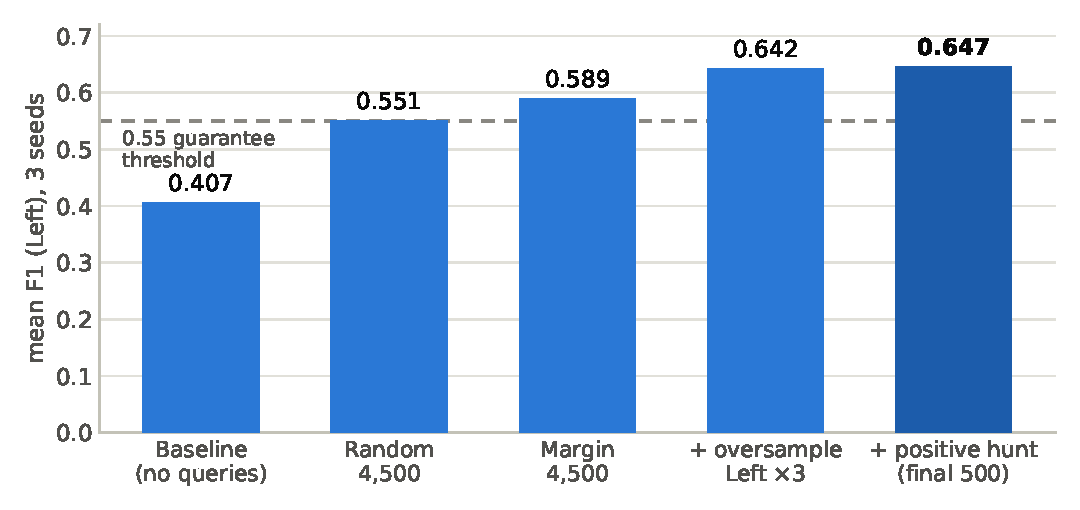
\includegraphics[height=46mm]{fig1_ablation.pdf}

{\small\textcolor{ink2}{Oversampling is the single biggest win (+0.053), for zero extra budget.}}
\end{center}
\slidefoot{3}
\newpage

% ── Slide 4 — Speaker 2 ──────────────────────────────────────────────────────
\slidetitle{Why $\times$3? The Oversampling Factor Is a Threshold Dial}
\begin{center}
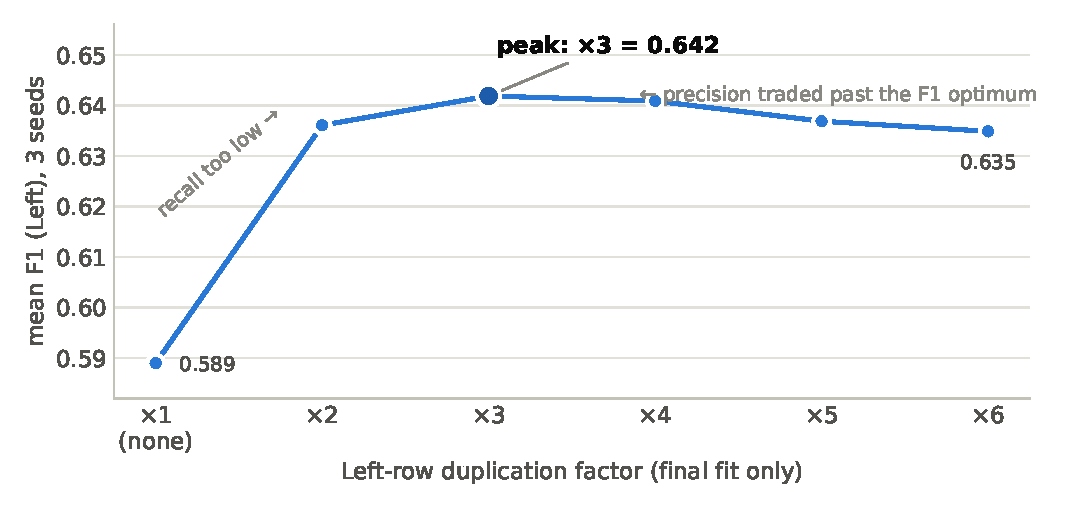
\includegraphics[height=39mm]{fig2_factor.pdf}

{\small\textcolor{ink2}{RF hyperparameters and encoding are fixed by the framework ---
the training distribution is our only tuning lever.\\
Duplication shifts the fixed 0.5 threshold implicitly; F1 peaks at $\times$3.}}
\end{center}
\slidefoot{4}
\newpage

% ── Slide 5 — Speaker 3 ──────────────────────────────────────────────────────
\slidetitle{What Did Not Work --- and Why}
\begin{center}
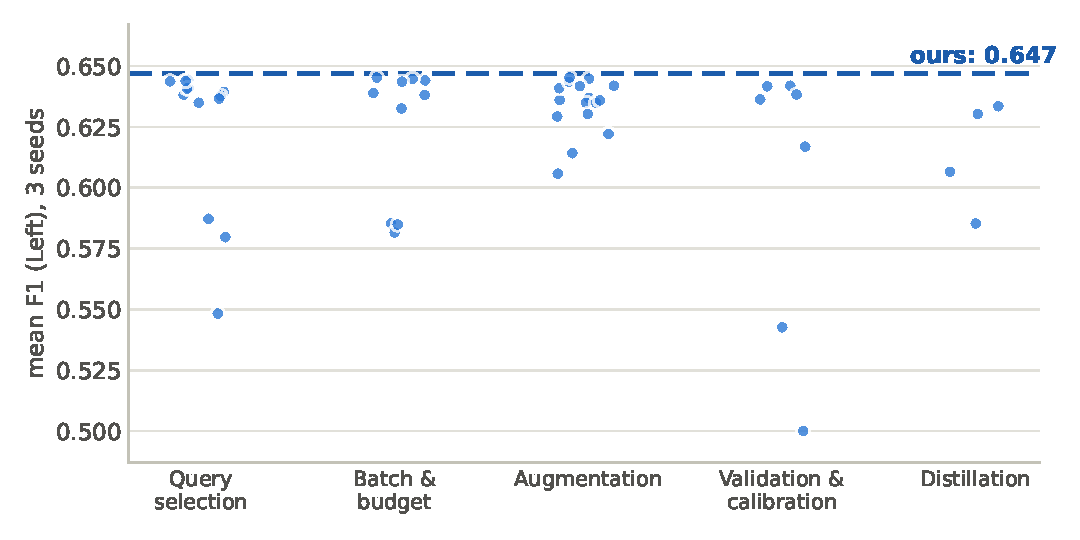
\includegraphics[height=40mm]{fig3_rejected.pdf}

\colorbox{panel}{\begin{minipage}{0.9\linewidth}\vspace{0.5ex}\centering
{\small\textcolor{ink}{\textbf{Key finding:} after querying, the training set is
$\sim$51\% positive vs.\ $\sim$33\% in the pool ---
so any hyperparameter validated on queried data does not transfer.}}
\vspace{0.5ex}\end{minipage}}
\end{center}
\slidefoot{5}
\newpage

% ── Slide 6 — Speaker 3 ──────────────────────────────────────────────────────
\slidetitle{Results \& Conclusion}
\vspace{1ex}
\begin{center}
\begin{tabular}{lcccc}
  \toprule
  & Seed 1 & Seed 2 & Seed 3 & \textbf{Mean} \\
  \midrule
  F1 (Left) & 0.6383 & 0.6493 & 0.6535 & \textbf{\textcolor{blueem}{0.6470}} \\
  \bottomrule
\end{tabular}
\end{center}

\vspace{1.5ex}
\renewcommand{\labelitemi}{\textcolor{blue1}{\raisebox{0.25ex}{\scriptsize$\bullet$}}}
\begin{itemize}\setlength{\itemsep}{0.6ex}
  \item Runtime 20--30\,s of the 60\,s budget per seed
  \item Top alternatives sit within seed-level noise ($\pm$0.005--0.01)
  \item Stopped after 3 passes --- further local search would overfit the local test sets
\end{itemize}

\vspace{1.5ex}
\begin{center}
{\large\textbf{Simple, budget-aware components beat every clever variant we tried.}}
\end{center}
\slidefoot{6}

\]
\end{document}